\chapter{Evaluation}
\label{cha:evaluation}

In this chapter, the quality of two selected toolkits is examined based on the requirements that were defined in Chapter~\ref{cha:requirements}. The basic goal is to show strengths and weaknesses of existing solutions with the aim to to give visualization authors the chance to pick the right tool for a certain task. This evaluation is used to examine the quality of Unveil.js, the author's contribution to the set of available visualization toolkits. The result should give information about whether the design goals have been met or not. D3.js has been selected for comparison, since it uses a fundamentally different strategy for solving the same sort of problems (animation, interaction). The comparison of these two frameworks drives a discussion about strengths and weaknesses of each approach. Additionally, a benchmark has been implemented for the comparison of rendering performance.

\section{Methodology}
%%%-----------------------------------------------------------------------------

Because of the versatile characteristics of programming languages, visualizations toolkits and visualizations in general the following discourse does not claim to be an exact evaluation of quantitative measures telling the true quality of certain solutions. There is no meaningful approach to determine the exact value of examined toolkits based on quantitative measures. In our evaluation, toolkits receive scores for each requirement. 

% In order to allow a refined total score we use different weights (Figure~\ref{tab:weighting}) for the requirements, as their individual importance for the overall qualification differs.

% \subsection{Scoring System}
%%%-----------------------------------------------------------------------------

The possible scores (Figure~\ref{tab:scoring}) per requirement range from 0 (not supported or insufficient quality) to 3 (complete support or very high quality).

\begin{table}
\caption{Scoring System}
\label{tab:scoring}
\centering
\setlength{\tabcolsep}{5mm} % separator between columns
\def\arraystretch{1.25} % vertical stretch factor
\begin{tabular}{|r||c|c|c|} \hline
Score & \emph{Level of Support} & \emph{Quality}\\
\hline\hline
3 & complete & very high \\
\hline
2 & good & satisfying \\
\hline
1 & basic & sufficient \\
\hline
0 & not supported & insufficient \\
\hline
\end{tabular}
\end{table}


% \subsection{Weighting}
% %%%-----------------------------------------------------------------------------
% 
% Based on the explanations by Bostock and Heer~\cite{D3}, we use a higher weight for \textit{Declarative Language Design} and a lower weight for \textit{Cross-platform Deployment}, since our evaluation is dedicated to web-based deployment. In practice, when applying this evaluation framework, weights should be chosen with respect to the concrete evaluation task.


% \begin{table}
% \caption{Weighting of evaluation requirements}
% \label{tab:weighting}
% \centering
% \setlength{\tabcolsep}{5mm} % separator between columns
% \def\arraystretch{1.25} % vertical stretch factor
% \begin{tabular}{|r||c|c|c|} \hline
% \emph{Criterion}                         & \emph{Weight} \\
% \hline\hline
% Declarative Language Design              & 17\% \\
% \hline
% Cross-platform Deployment                & 5\% \\
% \hline
% Optimization                             & 13\% \\
% \hline
% Data Representation and Transformation   & 13\% \\
% \hline
% Object-oriented Composition              & 13\% \\
% \hline
% Interaction                              & 13\% \\
% \hline
% Animation                                & 13\% \\
% \hline
% Extensibility                            & 13\% \\
% \hline
% \end{tabular}
% \end{table}


\section{Unveil.js}
%%%-----------------------------------------------------------------------------

Unveil.js, as described in Chapter~\ref{cha:unveil}, is a data-driven visualization toolkit, providing a slim abstraction in the form of a Scene API on top of the HTML5 Canvas element.

\subsection{Declarative Language Design}
%%%-----------------------------------------------------------------------------

Unveil.js uses a declarative scene definition format based on JSON. Users can specify graphical objects, so called Actors, that appear in the scene as well as behavior like interaction with objects. Moreover, animated transitions can be specified by using a simple declarative API.

\SuperPar \textbf{Score: 3}

\subsection{Cross-platform Deployment}
%%%-----------------------------------------------------------------------------

Unveil.js uses a toolkit-specific specification syntax for describing visualizations. By separating specification from execution, it is suitable for retargeting to other platforms. However, Unveil.js is an embedded DSL hosted by the Javascript programming language. This implies that porting it to other platforms is constrained to the Javascript scripting environment. Given that Javascript is available outside of the browser (Rhino\footnote{http://www.mozilla.org/rhino}, Node.js\footnote{http://nodejs.org}) visualizations can be retargeted to run in these environments.


\SuperPar \textbf{Score: 1}


\subsection{Optimization}
%%%-----------------------------------------------------------------------------

Since visualization specification is decoupled from implementation, optimizations can be applied by the language designer~\cite{DeclarativeLD10}. There are many options for optimization, such as improving the evaluation and rendering stages. With some effort, supporting new rendering platforms (such as WebGL) is also possible without changing the scene definition language.

\SuperPar \textbf{Score: 3}

\subsection{Data Representation and Transformation}
%%%-----------------------------------------------------------------------------

Unveil.js comes with extended support for data representation and transformation. Through Data.js it supports data abstraction formats for both tabular data (\texttt{Data.Collection}) and linked data (\texttt{Data.Graph}). Unveil.js promotes the creation of highly data-driven visualizations, which can not only use raw data but also meta-data, giving information about how a particular dataset is structured.

\SuperPar \textbf{Score: 3}

\subsection{Object-oriented Composition}
%%%-----------------------------------------------------------------------------

Unveil.js features some pre-implemented graphical objects (Actors). The object-oriented design should encourage users to think in graphical objects, which makes the process of creating complex visualizations easier. New customized Actors can be derived from existing actors or aggregate lower level actors to higher level ones that form reusable modules. In Unveil.js, the creation of new actors is a fundamental part of the visualization creation process.

\SuperPar \textbf{Score: 3}

\subsection{Interaction}
%%%-----------------------------------------------------------------------------

Unveil.js provides support for event handlers that can be bound to graphical objects. With the regular Canvas API this would not be possible because graphical objects are not tracked. In order enable interaction, hit testing, based on \texttt{isPointiInPath}, must be implemented for each Actor. In terms of performance, Unveil.js detects if interaction could potentially happen (e.g. when the mouse cursor is moved) and allocates resources (in the form of an increased frame rate) only on demand. For custom objects, however, users need to specify a corresponding bounding box themselves, which can be difficult and time-consuming for complex forms.

\SuperPar \textbf{Score: 2}

\subsection{Animation}
%%%-----------------------------------------------------------------------------

Unveil.js adds support for animation of graphical properties through the \texttt{animate} method provided by Actors. 

As it is the case with interaction, the frame rate of the visualization becomes increased only demand to keep overall CPU utilization low. Since the HTML5 Canvas element is used for rendering, Unveil.js is suitable for simultaneously animating large numbers of objects.

\SuperPar \textbf{Score: 3}

\subsection{Extensibility}
%%%-----------------------------------------------------------------------------

Extensibility is realized through the Actor abstraction, that enables users to compose higher level objects. These objects are derived from or composed of lower level graphical primitives. Actors can be used not only for graphical primitives but also for abstracting real world objects (carrying data and state) and encapsulating interaction and animation.

\SuperPar \textbf{Score: 3}


\section{D3.js}
%%%-----------------------------------------------------------------------------

D3.js is similar to its predecessor Protovis and offers comparable notational efficiency but differs in the method of implementation as the native representation (DOM) is directly exposed by the interface.

\subsection{Declarative Language Design}
%%%-----------------------------------------------------------------------------

D3 provides a declarative interface for specifying document transformations based on data. While Protovis focussed on the specification of static scenes, D3 offers an interface for specifying dynamic visualizations involving animation and interaction. In order to utilize the notational efficiency of specialized graphical primitives that are not offered by SVG directly, the \texttt{d3.svg} module provides various shapes suitable for charting. 

\SuperPar \textbf{Score: 3}

\subsection{Cross-platform Deployment}
%%%-----------------------------------------------------------------------------

D3 uses a representation transparent approach and relies on the document object model, and thus on web-native technologies (HTML, SVG and CSS). Consequently, this implies that visualizations specified using D3~\cite{D3} cannot be deployed to platforms other than the web. This is by design, according to Michael Bostock, and in turn offers better accessibility, while transformations of the DOM offer dramatic performance gains.

\SuperPar \textbf{Score: 0}

\subsection{Optimization}
%%%-----------------------------------------------------------------------------

The result of D3 document transformations is a scene graph, represented as DOM elements. Overall visualization performance depends on the performance offered by browsers. There is no intermediate representation (such as a toolkit-specific scene graph) that could be optimized in terms of evaluation or rendering. This is all up to the native browser technologies, such as Javascript, SVG and CSS. Because the DOM is modified directly, D3 can avoid unnecessary computation, as transformations can be limited to selected attributes. The author assigns a score of 2 here, as D3.js performance can be considered good. However, the design of this library intentionally does not offer much room for rendering optimization.

\SuperPar \textbf{Score: 2}

\subsection{Data Representation and Transformation}
%%%-----------------------------------------------------------------------------

D3 works with Javascript-native data structures, such as arrays and objects. There are a number of utility functions available, e.g. for working with dates, scales and colors. D3, however, lacks support for higher level data-abstraction. Since Data.js is available as a separate library, D3 users could use it to fill this gap.

\SuperPar \textbf{Score: 1}

\subsection{Object-oriented Composition}
%%%-----------------------------------------------------------------------------

As a consequence of not introducing a scene graph abstraction, D3.js lacks an object oriented interface. An object-oriented programming model often helps with thinking and abstracting from real world objects. D3.js gives users full freedom about how they can structure their code and fits well into the Javascript programming model. However, depending on the programming background of the user it might complicate learning the language and dealing with complex visualization tasks.

\SuperPar \textbf{Score: 0}


\subsection{Interaction}
%%%-----------------------------------------------------------------------------

With D3, adding interaction is easy. Because the DOM is exposed, event handlers can be attached to graphical objects directly. Programmers, who have done web-development or have used DOM manipulation libraries such as jQuery\footnote{http://jquery.com/} will immediately be familiar with it. D3 also makes data objects available to event handlers, allowing data-driven interaction.

\SuperPar \textbf{Score: 3}

\subsection{Animation}
%%%-----------------------------------------------------------------------------

Being the official successor of Protovis, D3.js comes with comprehensive support for transitions, where attributes or styles are smoothly interpolated over time. Animated transitions can be specified using the transition operator. There is support for staggered animation through individual specification of delay and duration. The easing method can be customized too. Performance experiments have shown that animation works well with a moderate number of motion tweens running at the same time. If the number of animated objects become too high, rendering performance drops significantly. In such scenarios, the Canvas Rendering API has some advantages.

\SuperPar \textbf{Score: 3}

\subsection{Extensibility}
%%%-----------------------------------------------------------------------------

D3 can be extended through optional modules which can be included as needed without bloating the library's core. There are numerous modules available, such as the \texttt{geo} module, which adds support for geographic data or the \texttt{geom} module, which adds computational geometry utilities (e.g. layout algorithms). Moreover, the layout module is an important one, as it is providing various reusable visualization layouts, such as force-directed graphs, treemaps and chord diagrams. The module system can be used by D3.js users to build extensions that can easily be adapted by others.

\SuperPar \textbf{Score: 3}


\section{Performance Evaluation}

In addition to the qualitative evaluation based on requirements, a performance benchmark has been implemented that opposes Unveil.js with D3.js. 
The benchmark considers initialization times and frame rates by constructing a scatterplot using different numbers of objects. The results, as shown in Figure~\ref{fig:benchmarks}, reveal that overall performance highly depends on the browser's implementation of native interfaces (HTML Canvas and SVG). Current webkit-based browsers (Google Chrome, Safari) provide high performance rendering for the SVG interface, which makes D3 noticeably faster here. Moreover profiling results have shown that Unveil.js performance (compared to native usage of the Canvas element) is decreased due to the application of matrix transformations. Unveil.js uses its own matrix library in order to let users adjust the object drawing order. However, this has been identified as a significant bottleneck and should be optimized in future.

In general both libraries offer sufficiently fast performance to implement interactive visualizations involving animation. Importantly, the results shown in the benchmark are just a snapshot considering a single use-case. According to the explanations in the qualitative evaluation, visualization designers need to decide themselves, which is the best solution for a particular task.

\begin{figure}
\centering
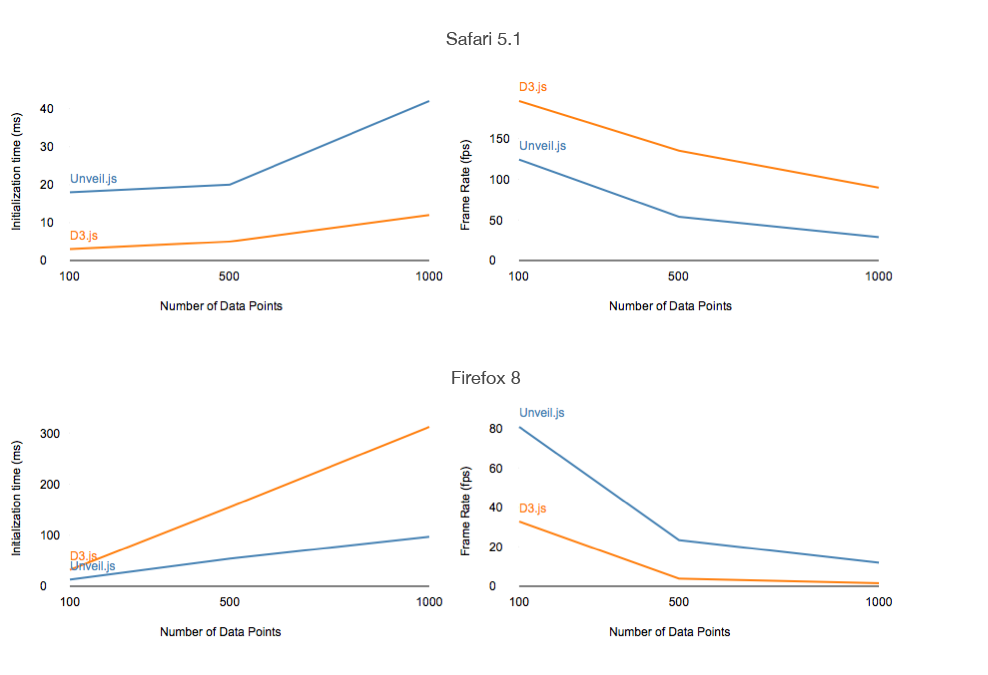
\includegraphics[width=1\textwidth]{benchmarks}
\caption{Performance benchmarks. Initialization times (left) and frames rates (right) for Safari (top) and Firefox (bottom).}
\label{fig:benchmarks}
\end{figure}



\section{Summary}

The toolkits examined both try to solve the same range of issues involving \emph{expressive methods of specification} and solutions for \emph{animation} and \emph{interaction}. D3.js, on the one hand, uses a representation transparent approach and intentionally abandons the possibility of cross-platform deployment. Instead, it focuses on providing a simplified interface to interact with web-native technology. Unveil.js, in turn, targets highly data-driven visualization tasks using a toolkit specific abstraction for describing scenes. It has its focus on modularization and code-reuse and uses an object-oriented approach to match the mental model of real world objects. 

\begin{table}
\caption{Comparison of individual scores between Unveil.js and D3.js}
\label{tab:comparison}
\centering
\setlength{\tabcolsep}{5mm} % separator between columns
\def\arraystretch{1.0} % vertical stretch factor
\begin{tabular}{|r||c|c|c|} \hline
\emph{Requirement} & \emph{Unveil.js} & \emph{D3.js}\\
\hline\hline
Declarative Language Design & 3 & 3\\
\hline
Cross-platform Deployment & 1 & 0\\
\hline
Optimization & 3 & 2\\
\hline
Data Representation and Transformation & 3 & 1 \\
\hline
Object-oriented Composition & 3 & 0 \\
\hline
Interaction & 2 & 3 \\
\hline
Animation & 3 & 3 \\
\hline
Extensibility & 3 & 3 \\
\hline
% Total Score &  & 2.77 & 2.07 \\
% \hline
\end{tabular}
\end{table}

% The scores do not reflect the overall quality of evaluated toolkits, they just emphasize the support of different requirements.

While D3's expressive syntax and deep integration with developer tools is suitable for many visualization tasks, Unveil.js may be a good fit when it comes to approaching complex visualization tasks through object-oriented abstraction.

In addition, Unveil.js contributes Data.js, a comprehensive data manipulation framework that offers a programmatic interface to domain data.